\chapter{Evaluation}
\label{evaluation}
%What systems do we chose to show our evaluation on and why?
%Why are they important
%How are they different from each other?
%Why does my system selection show that our techniques are generalizable. 
Table \ref{tab:table1} presents the architectures of the three \ac{DNN}s used in \ac{APS}, \ac{HCAS}, and \ac{ACAS-Xu}, in increasing order of complexity. 
These applications are all mission critical and can produce catastrophic outcomes in the presence of a successful attack.
They also come from two rather different domains: medical devices and autonomous vehicles, providing evidence of the generality of \tool. 

%We test our approach to incrementally larger DNNs. Larger DNNs imply networks with more layers and neurons per layer. %As mentioned previously, we have tested our approach for feed-forward neural networks that use ReLU for adding non-linearity. 


\begin{table}[h!]
	\begin{center}
		\caption{System descriptions}
		\label{tab:table1}
		\begin{tabular}{l|S|r|l}
			\textbf{} & \textbf{APS} & \textbf{HCAS} & \textbf{ACAS-Xu} \\
			%$\alpha$ & $\beta$ & $\gamma$ & $\gamma$ \\
			\hline
			\textbf{Size of the networks} &  &  &  \\
			Number of inputs &  74&   5&  5\\
			Number of hidden layers &  2&  3&  3\\
			Neurons/Layer &  8&  25 & 50 \\
			Number of outputs & 1&  5& 5\\
			\hline
			\hline
			
			%\textbf{Attacks synthesis (Avg. time in secs.)} &  &  &  \\
			%FDI attacks by perturbing 1 input &  0.01&  1000 &2700 \\
			%    FDI attacks by perturbing 2 inputs &  < 1&  2200&3600 \\
			%    FDI attacks by perturbing all inputs &  < 1&  2500& 5400 \\
			%    FDI attacks by perturbing 4 inputs  & &  & \\
			%    \hline
			%    \hline
		\end{tabular}
	\end{center}
\end{table}




We chose safety-critical applications for evaluating our approach. 
Our first application was inspired by the open-source system called openAPS.
Dutta et al. \cite{10.1007/978-3-319-99429-1_11} proposed a DNN for APS that takes in 74 inputs by discretizing time.
The second and third systems are modeling a collision avoidance (CA) system; it is a automatic system designed for unmanned vehicles  
The researchers proposed ACAS Xu standards that are tailored for threat CA logic and horizontal logic \cite{7778055}. 
These standards were implemented in \ac{ACAS-Xu} \ac{DNN}.
There are 45 DNNs that together make up the collision avoidance system \cite{Julian_2019}.  
Julian et al. \cite{Julian_2019} proposed a DNN compression for ACAS by representing large data tables in the form of DNNs. ACAS Xu dataset is currently proprietary and hence we did not have access to it. But for our tool, the trained model is enough to synthesize \ac{FDIA}. \ac{HCAS} is an open-source model created for collision avoidance. The reason we test our approach on ACAS and HCAS is that the sizes of these systems are different. The cost functions designed are the same in both cases.

\section{Methodology}
Our overall methodology is described in Figure \ref{fig:methodology-2} which describes how we evaluate three different systems. 
We pass the trained \ac{DNN} models through our tool which then synthesizes the critical inputs and the perturbations for conducting \ac{RFDIA} if they exist. 
Our tool currently supports tensorflow and pytorch formats.

As explained in \ref{relusyn} the tool converts the \ac{DNN} to \ac{MILP} format and provides the critical inputs and the perturbations. 


We used an 8-core system and ran the experiments on Gurobi such that it uses a single thread for running the experiments. 

Using this approach the attacker can use \tool to synthesize the attacks and can mount the attacks on these systems in real-time by introducing noise in the physical and/or network communications as explained in Chapter ~\ref{attack}. 
Our work focuses on synthesizing the attacks if they exist and not the latter part. 



\begin{figure}
	\centering
	\includegraphics[width=0.7\linewidth]{"Images/Methodology2"}
	\caption[Methodology]{Our work supports DNNs modeled in tensorflow and pytorch. These files when passed through ReLUSyn produce the critical inputs and perturbations that can be used to conduct ripplle false data injection attacks if they exist.}
	\label{fig:methodology-2}
\end{figure}



\section{APS}
%The APS model designed by Kushner et al. \cite{Dutta_Others__2018__Robust}\smi{add space here}is a data-driven model. The goal of the model is to predict future blood glucose values for the patients.
APS is the running example that we have used throughout the paper. 
APS model predicts the insulin value at a "lookahead" time $t + T$, using the history of the past $N$ glucose and insulin values with a step size of $h$. 
The step size implies that the data is recorded after every $h$ seconds from the starting time. The inputs contain the past insulin values and glucose values by keeping the step size $h$ as 5 and the neural network builds the mapping between input and output values. It is a network with two hidden layers (with 8 neurons per layer), 74 inputs and one output that predicts the future insulin values. 

%Attacks in the APS system.
Using \tool, we can successfully synthesize attacks in less than a minute. 
%The experiments that we conduct



\begin{table}[h!]
	\begin{center}
		\caption{Critical Inputs - APS - 1 Input perturbed at a time}
		\label{criticalinputs}
		\begin{tabular}{l|S|r}
			\textbf{Output range} & \textbf{Total inputs} & \textbf{Critical Inputs}  \\
			%$\alpha$ & $\beta$ & $\gamma$ & $\gamma$ \\
			\hline
			(204 $<= Output <=$ 210) &  74&  (1-5, 7, 9-13, 34-43,45,70-74) \\
			
		
			(210 $<= Output <=$ 215) &  74&   (41, 43)\\
			(215 $<= Output <=$ 220) &  74&  X \\
			(220 $<= Output <=$ 221) &  74&  X \\
			%(200 <= Output <= 203) &  74& , 50, 51, 53, 54, 55, 56, 59, 60, 61, 62, 63, 64, 65, 66, 67, 68, 69, 70, 72, 73) \\
			(200 $<= Output <=$ 203) &  74&  (23, 31, 35, 36, 38-41, 42, 45-51, 53-56, 59-70, 72, 73) \\
			(197 $<= Output <=$200) & 74& (40, 45, 48-51, 56, 61, 63-67, 70, 72, 73)\\
			\hline
			\hline
			
		
		\end{tabular}
	\end{center}
\end{table}


\begin{table}[h!]
	%\centering
	\caption{APS Results: The Attack column consists of the attack models where our goal is to minimize the inputs, Output ranges are the output bounds we have set where we want to find the deltas, no. of combinations is the combinations of attacks depending on the attack model (APS has 74 inputs) which is followed the total number of successful and unsuccessful attacks, peak time to conduct an attack in each set of experiment, memory used. }
	\label{APS}
	\begin{tabular}{|L{2cm}|L{2.7cm}|L{1cm}|L{1cm}|L{1cm}|L{1cm}|L{1cm}|L{4cm}|L{1cm}|}
		Attack & Output ranges (O) & No. of combinations  & Successful Attack(s) & Unsuccessful Attack(s) & Peak time& Memory used \\
		\hline
		
		\multicolumn{4}{c}{Attack 1: (-5 $<=$ Input $<$= 5)}\\
		\hline
		%\textbf{HCAS}&  &   & \\
		1 input changed at a time; delta minimization is primary objective& (204 $<$ O $<$ 210) \newline
		(210 $<$ O $<$ 215) \newline
		(215 $<$ O $<$ 220) \newline
		(220 $<$ O $<$ 221) \newline
		(200 $<$ O $<$ 203) \newline
		(197 $<$ O $<$ 200) \newline
		(194 $<$ O $<$ 197)& 74 \newline
		74 \newline
		74 \newline
		74 \newline
		74 \newline
		74 \newline
		74&   60 \newline
		2 \newline
		0 \newline
		0 \newline
		34 \newline
		16 \newline
		8& 14 \newline
		72 \newline
		74 \newline
		74 \newline
		40 \newline
		58 \newline
		66& 0.009 \newline
		0.001 \newline
		0.001 \newline
		0.001 \newline
		0.018 \newline
		0.008 \newline
		0.001& 21.8 \newline
		18.2 \newline
		18.1 \newline
		18.2 \newline
		22.8 \newline
		22.2 \newline
		18.5  \\
		
		
		\hline
		\multicolumn{4}{c}{Attack 2: (-5 $<=$ Input $<$= 5)}\\
		\hline
		%\textbf{HCAS}&  &   & \\
		2 inputs changed at a time; delta minimization is primary objective&(204 $<$ O $<$ 210) \newline
		(210 $<$ O $<$ 215) \newline
		(215 $<$ O $<$ 220) \newline
		(220 $<$ O $<$ 221) \newline
		(200 $<$ O $<$ 203) \newline
		(197 $<$ O $<$ 200) \newline
		(194 $<$ O $<$ 197)&  2701 \newline
		2701 \newline
		2701 \newline
		2701  \newline
		2701  \newline
		2701 \newline
		2701& 2669 \newline
		220 \newline
		29 \newline
		2 \newline
		2142 \newline
		1374 \newline
		739&   32 \newline
		2481 \newline
		2672 \newline
		2699 \newline
		559 \newline
		1327 \newline
		1962& 0.029\newline
		0.0139 \newline
		0.006 \newline
		0.003 \newline
		0.0632 \newline
		0.0412  \newline
		0.0413 & 21.8
		18.2
		18.1
		18.2
		22.8
		22.2
		18.5\\
		
		\hline
		\multicolumn{4}{c}{Attack 3: (-5 $<=$ Input $<$= 5)}\\
		\hline
		%\textbf{HCAS}&  &   & \\
		74 (All) inputs changed at a time; delta minimization is primary objective&  (204 $<$ O $<$ 210) \newline
		(210 $<$ O $<$ 215) \newline
		(215 $<$ O $<$ 220) \newline
		(220 $<$ O $<$ 221) \newline
		(200 $<$ O $<$ 203) \newline
		(197 $<$ O $<$ 200) \newline
		(194 $<$ O $<$ 197)& 1 \newline
		1 \newline
		1 \newline
		1 \newline
		1 \newline
		1 \newline
		1&   1 \newline
		1 \newline
		1 \newline
		1 \newline
		1 \newline
		1 \newline
		1& 0 \newline
		0 \newline
		0 \newline
		0 \newline
		0 \newline
		0 \newline
		0& 0.037
		0.060
		0.049
		0.045
		0.110
		0.073
		0.062&23.1
		19.1
		20.3
		20.3
		22.5
		22.0 \newline
		23.0\\
		\hline
		
		
		
		
		
		
		
		
		
	\end{tabular}
\end{table}



\subsection{Attacks}
The goal is to minimize the input perturbations such that the output is perturbed by amounts so it remains between the user-specified lower and the upper bounds.
Injecting more than the required amounts even if within the bounds is potentially fatal for users of the systems. 

%Randomly changing inputs can trigger alarms in the system because it will raise the levels above the bounds enforced by specifications. We want to perturb the inputs in a stealthy way. The stealthiness is induced by finding the exact perturbations and to find those exact perturbations we need \tool. Brute force would require to search through the entire search space. We model the attack by including a $delta$ function in the inputs. 
To locate the critical inputs we first perturb the inputs, one at a time, to induce small perturbations in the outputs as shown in Table ~\ref{summary} under the APS section and in more details in Table ~\ref{APS}. 
We find that for different ranges of outputs, the critical inputs vary as shown in Table ~\ref{criticalinputs}. 
We have included the critical inputs when we perturb only one input at a time since these are the most useful from an attackers' perspective, and also because of space reasons. 
As we can observe in Table ~\ref{APS} as the number of perturbed inputs increases the possible combinations of critical inputs also increases. 



%, For example, we find that when we perturb one input for an output range of 194-197, changing any one of these (40, 50, 61, 63, 66, 67, 72, 73) inputs by certain amounts will result in a successful  FDI \attack. Due to space reasons, we provide a summary of all combinations of attacks in Table II for APS. 
%Along with the critical inputs, we also obtain the perturbations that will lead to an output deviation. 
%Further we try 

%We observe that it is feasible to find one input perturbation that can cause output perturbations without getting detected. We find every attack for APS within seconds. We test out our approach by perturbing specific inputs at a time instead of randomly finding attacks. 

%We generate attacks by keeping all inputs constant but one to observe the above phenomenon. We keep all inputs constant but two in the next set of the experiment to understand if it is easier to find such attacks as compared to finding only one input perturbation and in the process, we are successfully able to locate the critical inputs.  






%Table template
\iffalse
\begin{table}[h!]
	%\centering
	\caption{Results Summary}
	%\label{summary}
	\begin{tabular}{l|S|r|l|r|l|r|l}
		Attack & Attack  & No. of  & Successful & Unsuccessful  & Peak  & Memory \\
		&  No. &  combinations &  Attack(s) & Attack(s& time& used \\
		\hline
		
		\multicolumn{4}{c}{Random}\\
		\hline
		%\textbf{HCAS}&  &   & \\
		&  & &   & & &\\
		&  & &   & & &\\
		
		\hline
		\multicolumn{4}{c}{Targeted}\\ 
		\hline
		
		
	\end{tabular}
\end{table}
\fi

%\section{FDI attack 2}
%In our next set of attacks we maximize the output deviation and minimize the input deviations. We do so to cause the maximum damage possible to a patient by perturbing inputs within bounds yet we want it to perturb by maximum amounts within those bounds. As shown in Table 2  in the lower half we conduct a similar analysis by keeping everything constant but perturbing on 1, 2 and then finally all inputs together. We conduct these experiments to show that our technique is capable of identifying one critical input and also a set of critical inputs that can cause output deviations. 



\section{ACAS Xu and HCAS}




\begin{table}[h!]
	%\centering
	\caption{HCAS Results: The different attacks are explained in the Attack column which depends on the order of the outputs and the ranges of the deltas, the number of inputs to be perturbed are selected by the attacker for  conducting each attack, the total number of combinations are calculated based on the total number of inputs  and the inputs selected to be perturbed, the peak time is the maximum time it took to test for an attack from the combinations, X indicates that the experiments timed out.}
	\label{hcas}

		\begin{tabular}{|L{3cm}|L{2cm}|L{1cm}|L{1cm}|L{1cm}|L{1cm}|L{1cm}|L{2cm}|L{1cm}|}
		Attack & Inputs perturbed & No. of combinations  & Successful Attack(s) & Unsuccessful Attack(s) & Peak time& Memory used &Critical inputs\\
		\hline
		
		\multicolumn{4}{c}{Random}\\
		\hline
		%\textbf{HCAS}&  &   & \\
		Attack 1 - One output is set to be minimum (others can be ordered arbitrarily); deltas are restricted to be 5 at the max and are minimized& 1A - 1 input
		1B - 2 inputs
		1C - 3 inputs & 12 \newline
		12 \newline
		4&   5 \newline
		11 \newline
		4& 7 \newline
		1 \newline
		0& 5.7 \newline
		94.3 \newline
		80.9& 70.2 \newline
		108 \newline
		103.5 & {0: [(0), (2)], 2: [(1)], 4: [(0), (1)]} \newline All but {1: [(1,2)]} 
		\\
		
		
		\hline
		\multicolumn{4}{c}{Targeted 1}\\ 
		\hline
			Attack 1 - Complete ordering on outputs; deltas do not have user-specified restriction and are not minimized &
			1A - 1 input
			1B - 2 inputs
			1C - 3 inputs& 3 \newline
			3\newline
			1 & 0\newline
			0\newline
			0&  3\newline
			3\newline
			1 &7.9 \newline
			174.4 \newline
			1130.6& 73.1 \newline
			114.9 \newline
			152.7 & NA\\
			
	 	\hline
	 \multicolumn{4}{c}{Targeted 2}\\ 
	 \hline
	 Attack 2 - Complete ordering on outputs; deltas do not have user-specified restriction and are not minimized&  2A - 1 input
	 2B - 2 inputs
	 2C - 3 inputs& 3 \newline
	 3 \newline
	 1&   0 \newline
	 0 \newline
	 0& 3 \newline
	 3 \newline
	 1& 6.7 \newline
	 214.6 \newline
	 2039.2 &71.5 \newline
	 123.9 \newline
	 290.1 & NA\\    
	 
	 
	 
	 	 	\hline
	 \multicolumn{4}{c}{Targeted 3}\\ 
	 \hline
	 Attack 3 - Partial ordering on outputs; deltas do not have user-specified restriction and are not minimized&  3A - 1 input
	 3B - 2 inputs
	 3C - 3 inputs& 3 \newline
	 3 \newline
	 1&   2 \newline
	 3 \newline
	 1& 1 \newline
	 0 \newline
	 0& 3.0 \newline
	 4.2 \newline
	 2.7& 69.0 \newline
	 71.5 \newline
	 67.4 & [0], [2] \newline
	  ([0,1],[0,2], [1,2]) \newline
	 ([0,1,2])\\
	 \hline
	  	 
		
		
	\end{tabular}
\end{table}

\begin{table}[h!]
	%\centering
	\caption{HCAS Results continued}
	\label{hcas2}
	
	\begin{tabular}{|L{3cm}|L{2cm}|L{1cm}|L{1cm}|L{1cm}|L{1cm}|L{1cm}|L{2cm}|L{1cm}|}
	Attack & Inputs perturbed & No. of combinations  & Successful Attack(s) & Unsuccessful Attack(s) & Peak time& Memory used &Critical inputs\\
	\hline
		\multicolumn{4}{c}{Targeted 4}\\ 
		\hline
		Attack 4 - Partial ordering on outputs; deltas do not have user-specified restriction and are minimized& 4A - 1 input
		4B - 2 inputs
		4C - 3 inputs & 3 \newline
		3 \newline
		1&   2 \newline
		3 \newline
		1& 1 \newline
		0 \newline
		0& 1 \newline
		0 \newline
		0& 69.4 \newline
		83.1 \newline
		76 & ([0], [2]) \newline
		([0,1], [0,2], [1,2]) \newline
		([0,1,2]) \\
		\hline
		\multicolumn{4}{c}{Targeted 5}\\ 
		\hline
		Attack 5 - Partial ordering on outputs; deltas do not have user-specified restriction and are not minimized&  5A - 1 input
		5B - 2 inputs
		5C - 3 inputs& 3 \newline
		3 \newline
		1&   0 \newline
		0 \newline
		1& 3 \newline
		3 \newline
		0& 4.9 \newline
		229.6 \newline
		1.8& 69.7 \newline
		110.4 \newline
		58.9 & 
		X  \newline
		X \newline
		([0,1,2])\\
		
		\hline
		\multicolumn{4}{c}{Targeted 6}\\ 
		\hline
		Attack 6 - Partial ordering on outputs; deltas do not have user-specified restriction and are minimized &
		6A - 1 input
		6B - 2 inputs
		6C - 3 inputs&  3 \newline
		3 \newline
		1& 0 \newline
		0 \newline
		1&   
		3 \newline
		3 \newline
		0 &
		X \newline
		X \newline
		357.4&
		X \newline
		X \newline
		111.1& 
		X  \newline
		X \newline
		([0,1,2])\\
		
		\hline
		\multicolumn{4}{c}{Targeted 7}\\ 
		\hline
		Attack 7 - Partial ordering on outputs; deltas do not have user-specified restriction and are not minimized&  7A - 1 input
		7B - 2 inputs
		7C - 3 inputs& 3 \newline
		3 \newline
		1&   1 \newline
		3 \newline
		1& 2 \newline
		0 \newline
		0& 3.5 \newline
		24.8 \newline
		1.9& 67.9 \newline
		90.5 \newline
		62.0 & [1] \newline 
	([0,1], [0,2], [1,2]) \newline
		([0,1,2])\\
		
		\hline
	
		
		
		
	\end{tabular}
\end{table}

\begin{table}[h!]
	%\centering
	\caption{HCAS Results continued}
	\label{hcas3}
	
	\begin{tabular}{|L{3cm}|L{2cm}|L{1cm}|L{1cm}|L{1cm}|L{1cm}|L{1cm}|L{2cm}|L{1cm}|}
	Attack & Inputs perturbed & No. of combinations  & Successful Attack(s) & Unsuccessful Attack(s) & Peak time& Memory used &Critical inputs\\
	\hline
		\multicolumn{4}{c}{Targeted 8}\\ 
		\hline
		Attack 8 - Partial ordering on outputs; deltas do not have user-specified restriction and are minimized&  8A - 1 input
		8B - 2 inputs
		8C - 3 inputs& 3 \newline
		3 \newline
		1&  1 \newline
		3 \newline
		1 & 2 \newline
		0 \newline
		0& 3.5 \newline
		80.5 \newline
		67.9& 68.6 \newline
		104.4 \newline
		103.1 & [1] \newline
		([0,1], [0,2], [1,2])
		([0,1,2])\\
		
		\hline
		\multicolumn{4}{c}{Targeted 9}\\
		\hline
		%\textbf{HCAS}&  &   & \\
		Attack 9 - Partial ordering on outputs; deltas do not have user-specified restriction and are not minimized& 9A - 1 input
		9B - 2 inputs
		9C - 3 inputs & 3 \newline
		3 \newline
		1&  0 \newline
		1 \newline
		1 & 3 \newline
		2 \newline
		0& 6.3 \newline
		139.3 \newline
		314.1 & 67.3 \newline
		98.4 \newline
		126.6 & 
		X \newline
		([1,2]) \newline
		([0,1,2])\\
		
			\hline
		\multicolumn{4}{c}{Targeted 10}\\
		\hline
		Attack 10 - Partial ordering on outputs; deltas do not have user-specified restriction and are minimized &
		10A - 1 input \newline
		10B - 2 inputs \newline
		10C - 3 inputs&
		3 \newline
		3 \newline
		1&
		0 \newline
		1 \newline
		1&
		3 \newline
		2 \newline
		0&
		4.7 \newline
		85.0 \newline
		228.8&
		71.6 \newline
		92.7 \newline
		109.9 &
		X \newline
		([1,2]) \newline
		([0,1,2])\\
		\hline 
		
		
	\end{tabular}
\end{table}

\begin{table}[h!]
	%\centering
	\caption{ACAS-Xu Results: The different attacks are explained in the Attack column which depends on the order of the outputs and the ranges of the deltas, the number of inputs to be perturbed are selected by the attacker for  conducting each attack, the total number of combinations are calculated based on the total number of inputs  and the inputs selected to be perturbed, the peak time is the maximum time it took to test for an attack from the combinations, X indicates that the experiments timed out.}
	\label{acasxu}
		

	\begin{tabular}{|L{3cm}|L{2cm}|L{1cm}|L{1cm}|L{1cm}|L{1cm}|L{1cm}|l}
		Attack & Inputs perturbed & No. of combinations  & Successful Attack(s) & Unsuccessful Attack(s) & Peak time& Memory used\\
	
		\hline
		\multicolumn{4}{c}{Random}\\
		\hline
		%\textbf{HCAS}&  &   & \\
		One output is set to be minimum (others can be ordered arbitrarily); deltas are restricted to be 5 at the max and are minimized& 1A - 1 input
		1B - 2 inputs
		1C - 3 inputs
		1D - 4 inputs
		1E - 5 inputs & 
		20  \newline
		40  \newline
		40   \newline
		20   \newline 
		4&  2  \newline
		9 \newline
		12 \newline
		8 \newline
		2 &
		18 \newline
		31\newline
		28\newline
		12\newline
		2 & 465.8
		4141.1
		6644.9
		17637.9
		11528.4&
		160.7 \newline
		209.1 \newline
		269.1 \newline
		449.5 \newline
		348.2 \\
		
		
		
		
		
		\hline
		\multicolumn{4}{c}{Targeted}\\ 
		\hline
		Complete ordering on outputs; deltas are restricted to be 5 at the max and are minimized&  1A - 1 input
		1B - 2 inputs
		1C - 3 inputs
		1D - 4 inputs
		1E - 5 inputs& 5 \newline
		10 \newline
		10  \newline
		5 \newline
		1&  0 \newline
		0 \newline
		0 \newline
		0 \newline
		0 &5 \newline
		10 \newline
		10 \newline
		5 \newline
		1 & 739.4
		3678.1
		7296.6
		24041.9
		4434.7& 204.8
		202.6
		296
		562.1
		200.2\\
		
		
		\hline
		\multicolumn{4}{c}{Targeted}\\ 
		\hline
		
		Partial ordering on outputs; deltas are restricted to be 5 at the max and are minimized&  2A - 1 input
		2B - 2 inputs
		2C - 3 inputs
		2D - 4 inputs
		2E - 5 inputs& 5 \newline
		10  \newline
		10  \newline
		5  \newline
		1&  0  \newline
		0 \newline
		X \newline
		X \newline 
		0 &5 \newline
		10  \newline
		X \newline X \newline
		
		1 & 975.8
		3816.4
		X\newline
		
		X \newline
		4766.6& 223.2 \newline
		197.1 \newline
		X \newline
		X \newline
		
		218.6\\
		
		\hline
		\multicolumn{4}{c}{Targeted}\\ 
		\hline
		Attack 3 - Partial ordering on outputs; deltas are unrestricted	&  3A - 1 input
		3B - 2 inputs
		3C - 3 inputs
		3D - 4 inputs
		3E - 5 inputs&  5 \newline
		10 \newline
		10 \newline
		5 \newline
		1 &   0\newline
		1\newline
		X \newline
		X \newline
		1&5 \newline
		9 \newline
		X \newline
		X \newline
		0&
		1075.0
		62876.6
	X \newline
	X	\newline
		8311.2& 288.2
		1740.5
	X	\newline
	X	\newline
		1447.4 \\
		\hline
	\end{tabular}
\end{table}
%We test our approach on two other available systems that are collision avoidance (CA) as explained in the above section. 
The ACAS Xu and HCAS are different from each other in terms of their architectures and parameters as shown in Table ~\ref{tab:table1}. 
Apart from the difference between the weights, bias and the number of layers, the datasets used to produce the two are also quite different. 

%We conduct two random and targeted \attack \smi{this is singular but should perhaps be plural; good idea to skim the rest of the paper where \attack is used} in these systems, to understand how the systems\smi{this sentence is incomplete}
The ACAS Xu is designed to model a large lookup table that maps sensor readings to the decisions based on the readings or advisories. 

The geometry of the ACAS Xu is shown in Figure ~\ref{fig:acasxugeometry}.
The ownship is the unmanned vehicle with the \ac{CA} system and the intruder's goal is to crash with the ownship. 
There are five sensor readings:  (1) Distance from ownship to intruder, (2) Angle to the intruder relative to ownship heading direction, (3) Header angle to intruder relative to ownship heading direction, (4) Speed of ownship, and (5) Speed of intruder.  
The outputs represent five different possible advisories or decisions based on sensor readings: (1 )clear-of-conflict (COC), (2) weak right, (3) strong right, (4) weak left, and (5) strong right. 
The advisories goals is to avoid crashes of the ownship with the intruder; incase the two are getting too close, an action is taken that moves the two apart. 
Based on the inputs, the one with the least value is the advisory that is going to be the action to be taken by the system.  


We conduct two types of \ac{RFDIA} here: targeted and random, to understand how long it take to synthesize attacks. 
In targeted attacks, the attacker specifically chooses an output that has to be minimized and have to have the smallest values of the five possible outcomes.
This means that out of the five advisories listed above depending on the ownship and the intruder location that action is taken which moves the ownship away from the intruder and the one with the smallest value is the action supposed to be taken by the \ac{CA}.
The \ac{HCAS} works in a similar way except that it takes in three inputs instead of five. %Also, as shown in Table 1, the parameters are different for ACAS Xu and HCAS. 


\begin{figure}
	\centering
	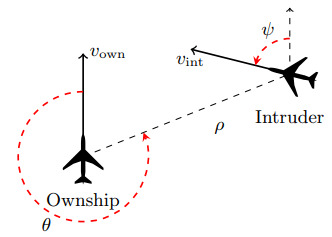
\includegraphics[width=0.7\linewidth]{Images/ACASXugeometry}
	\caption[ACAS Xu]{ACAS Xu geometry}
	\label{fig:acasxugeometry}
\end{figure}

\iffalse
%Explain about the normalization layer
The one feature about these systems that are different from the previous system which is the APS is that these systems consist of inputs and outputs normalization. These normalization are used to place bounds on how much the inputs can be perturbed by. To accommodate the normalization layer, we introduce certain heuristics that are deep network specific. %The normalization depends on the conditions that are introduced by the neural network.
\fi

We conduct two categories of attacks in \ac{ACAS-Xu} and \ac{HCAS}:
\subsection{Targeted attack} 
In the first attack, we minimize the input perturbations by keeping all but $1$, $2$ and $n$ inputs constant in the three sets of experiments that we conduct as shown in Table ~\ref{hcas}, ~\ref{hcas2}, ~\ref{hcas3} and ~\ref{acasxu} for \ac{HCAS} and \ac{ACAS-Xu}. 
Our goal is to find the smallest input perturbations that produce an output with the wrong direction, for instance, weak left to weak right, or weak right to weak left, or weak right instead of COC. 


Consider a set of five inputs for which the output is weak left. 
The output weak left indicates that the \ac{DNN} returns 4. 
The network is trained in a way such that the least value signifies the output that should be taken next. 
The attacker's goal is to change the output in a way such that the minimum value changes from weak left to weak right. 
To model this, we first add a delta value to the inputs as in our previous evaluation. 
To do so, we add constraints that force the output to 5 instead of 4; the constraints look of the form "$05 < $(All other outputs)".


Some combinations we experiment with are as follows:
\begin{enumerate}
	\item Targeted attack 1 = 03 $<$ 02 $<$ 01 $<$ 04 $<$ 05
	\item Targeted attack 2 = 03 $<$ 02 $<$ 01 $<$ 05 $<$ 04
	\item Targeted attack 3 = 01 $<$ 02 $<$ (any order)
	\item Targeted attack 4 = 01 $<$ (any order) 
\end{enumerate}
 
The attacker can conduct various targeted attacks using the critical inputs as shown in Table ~\ref{hcas}, ~\ref{hcas2}, ~\ref{hcas3} and ~\ref{acasxu} for \ac{HCAS} and \ac{ACAS-Xu} through physical means. 


\begin{figure}
	\centering
	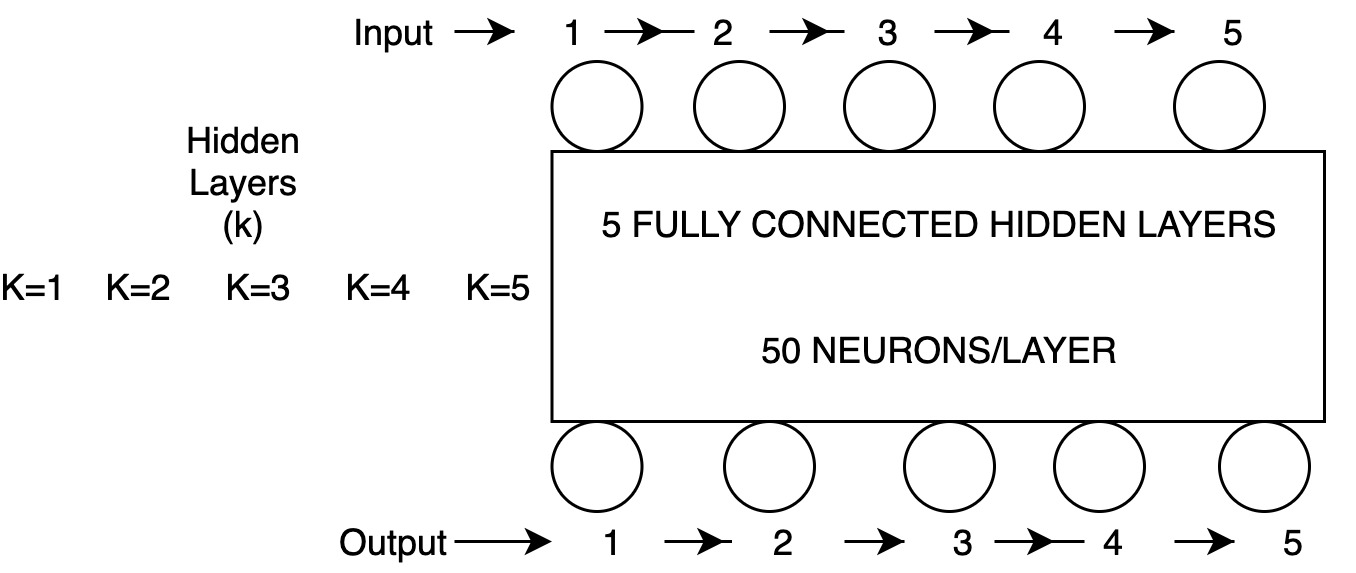
\includegraphics[width=0.7\linewidth]{Images/ACASXuDNN}
	\caption[ACAS Xu DNN]{ACAS Xu DNN representation: 5 inputs and 5 outputs with 5 hidden layers that consist of 50 neurons each.}
	\label{fig:acasxudnn}
\end{figure}

\subsection{FDI random attack} 
Constructing random \ac{RFDIA} attacks is slightly less effort for the attacker as compared to targeted attacks; this is because the constraints in a targeted setting are much tighter. 
Building on the previous example, if we have 5 inputs that give us the result as output 4, we need to perturb the inputs such that the output changes to any of the other possibilities such as output 1, output 2, output 3 and output 5.

In this case, we try out multiple different combinations that allow us to find the perturbations as shown in Table ~\ref{hcas}, ~\ref{hcas2}, ~\ref{hcas3} and ~\ref{acasxu} for \ac{HCAS} and \ac{ACAS-Xu}.



\section{Summary}
From our experimentation we conduct ~19,000 attacks for \ac{APS} out of which ~7200 attacks were successful and took less than 1 second. 
We conducted ~30 \ac{HCAS} random attacks out of which ~20 were successful and the maximum amount taken by the attacks was 41 seconds. 
We conducted ~7 targeted attacks for \ac{HCAS} out of which 1 attack was successful.
We conducted ~140 \ac{ACAS-Xu} random attacks out of which ~32 were successful and the maximum amount taken by the attacks was 7228 seconds. 
We conducted ~16 targeted attacks for \ac{HCAS} out of which 2 attacks was successful.
These results are shown in Table ~\ref{summary}.

Thus we can see that synthesizing \ac{RFDIA} attacks can be easily accomplished by the attacker in a small amount of time. 
We have also tried out multiple different combinations of attacks keeping multiple attacker scenarios in mind and show that for systems such as \ac{APS} perturbing a single input out of the 74 inputs is enough to cause damage in Table ~\ref{APS}.
Similarly for \ac{HCAS} and \ac{ACAS-Xu} we observe  from Table ~\ref{hcas}, ~\ref{hcas2}, ~\ref{hcas3} and ~\ref{acasxu} that perturbing a single input in certain scenarios is enough to cause output deviation. 

 \begin{table}[h!]
 	%\centering
 	\caption{Results Summary}
 	\label{summary}
 	\begin{tabular}{l|S|r|l}
 		\textbf{Inputs-pert} & \textbf{Total} &  \textbf{Successful} & \textbf{Mean-Time/ } \\
 		urbed/Attack &  Attacks &  Attacks &  Attack(s) \\
 		\hline
 		\multicolumn{4}{c}{APS}\\
 		\hline
 		1 &  518& 120 &  0.0015\\
 		2 &  18907& 7175 &  0.002\\
 		74 &  7& 7 &  0.03\\
 		\hline
 		\multicolumn{4}{c}{HCAS - Random}\\
 		\hline
 		%\textbf{HCAS}&  &   & \\
 		1 &  12& 5 &  3.87\\
 		2 &  12& 11 &  32.89\\
 		3 &  4&  4&  41.14\\
 		\hline
 		\multicolumn{4}{c}{HCAS - Targeted (Partial Ordering)}\\
 		\hline
 		%\textbf{HCAS}&  &   & \\
 		1 &  3& 1&  2.14\\
 		2 &  3& 0 &  2.91\\
 		3 &  1&  0&  2.74\\
 		\hline
 		\multicolumn{4}{c}{ACAS Xu - Random}\\
 		\hline
 		%\textbf{HCAS}&  &   & \\
 		1 &  20& 2&  100.11\\
 		2 &  40& 9& 548.72\\
 		3 &  40& 12&  1452.176\\
 		4 &  20&  8&  5029.58\\
 		5 &  20&  2&  7228.966\\
 		\hline
 		\multicolumn{4}{c}{ACAS Xu- Targeted (Partial Ordering)}\\ 
 		\hline
 		%\textbf{HCAS}&  &   & \\
 		1 &  5& 0&  297.2\\
 		2 &  10& 1 &  23595.58\\
 		5 &  1&  1&  8311.21\\
 		\hline
 		\hline
 	\end{tabular}
 \end{table}
